\chapter{Development of a Web-Based Visualization Tool for the Comparison of Organism Genome Properties} \label{micromeda-client}

As discussed in Chapter XXX, Micromeda's user interface is provided by a client web application. Its role is to provide users with a streamlined interface for visualizing patterns of genome property and step assignment across organisms. This assignment data is provided to the client in the form of user uploaded Micromeda files (Section XXX). After upload, these files are sent to Micromeda-Server (Chapter XXX) where they parsed and are used provide data to the client. The client can request this data through series of web API endpoints (Section \ref{endpoints}) provided by Micromeda-Server. In this chapter we will discuss the client web application, called Micromeda-Client, in detail.

\section{Visualisation Design}

One of the core uses of Genome Properties assignment data is to mine it for biologically relevant patterns in the presence and absence of biochemical pathways or structural features. One of the best ways to detect such patterns is through the use of data visualisation. By visualising such data we can make many types types of comparisons. Some example comparisons and their research relevance can be seen is Fig. \ref{fig:client-analysis-types} and the list below.

\begin{itemize}
\item Looking at the assignments of a single property across organisms can be used to used for the selection of subsets of organisms which may posses a specific phenotype (Fig. \ref{fig:client-analysis-types}a). In the field of genetic engineering, such comparisons could be used for host or gene donor selection.
\item Comparing the assignments of multiple properties could be used for identifying patterns of property conservation across organisms in a dataset (Fig. \ref{fig:client-analysis-types}c). In microbial ecology, such comparisons could be used to identify microorganisms which fit specific ecological niches.
\item Looking at the steps assignments of a single property in a single organism could be used to evaluate the correctness of the property's assignment in this organism  (Fig. \ref{fig:client-analysis-types}b). For example, a property might be assigned NO or PARTIAL because it is only missing a few required step assignments but possess many others (Fig. \ref{fig:client-analysis-types}b). Being able to look at all step assignments for the property may be useful for why a property has been given an assignment.
\item Comparing the step assignments of single property across organisms can be used to see what pathway steps are retained across organisms that differ photogenically (Fig. \ref{fig:client-analysis-types}d). For example, if a property step is not retained in a large assortment of genomes, it may not be required or is carried out by proteins which are non-canonical (Fig. \ref{fig:client-analysis-types}d). Such proteins may not posses domains used by Genome Properties but may still carry out the pathways step.
\end{itemize}

\begin{figure}[!ht]
  \centering
	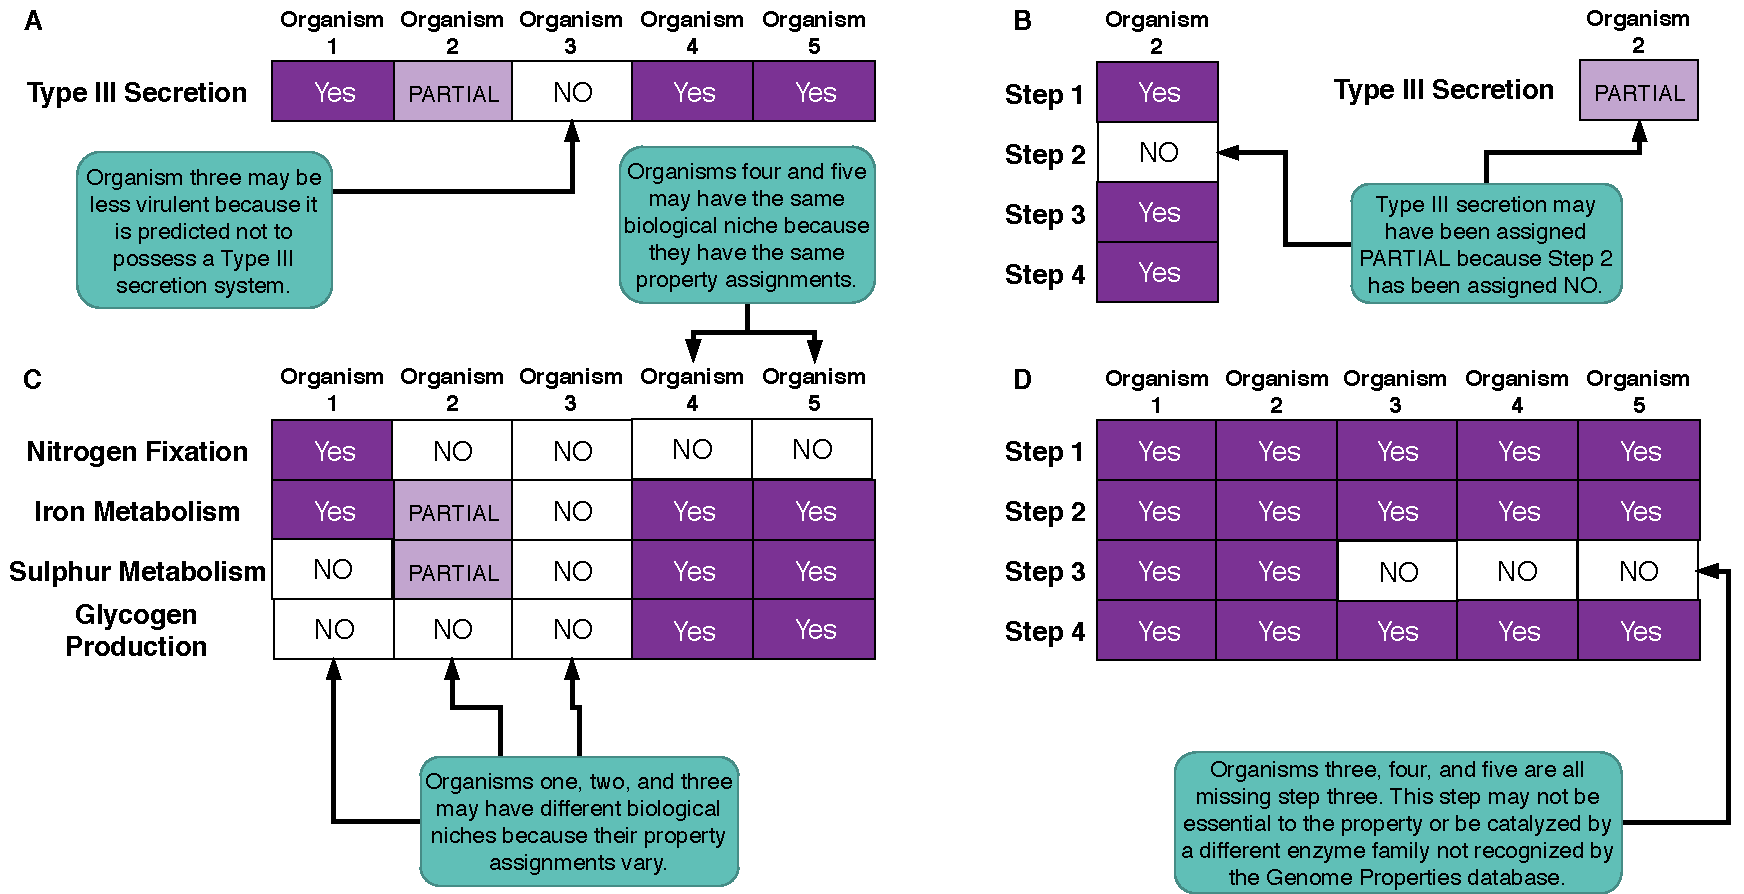
\includegraphics[width=\textwidth]{media/analysis_types.pdf}
	 \caption{Visualizations of Genome Properties data can be used to compare property and step assignments across organisms.}
	 \label{fig:client-analysis-types}
\end{figure}

If Micromeda-Client is to support the above comparison's, the data visualization method used Micromeda-Client should allow users to perform the following tasks.

\begin{itemize}
\item Track assignments across organisms.
\item Assess the magnitude of given assignments.
\item Aggregate step and property assignments into summaries.
\item Explore how these aggregate assignments are derived.
\item Quickly find assignments of interest.
\end{itemize}

When a visualization approach was select for use by Micromeda-Client, the compatibility of the visualization with these tasks was kept in mind.

\subsection{An Overview of Genome Properties Data}

Different types of data are more suitable to specific visualisation techniques and it is important to first discuss the nature of genome properties data before discussing why the author selected a specific type visualisation for Micromeda-Client. At its core the data presented by Micromeda-Client consists of assignments for properties and steps. Such assignments are ordinal data \cite{richardson2018genome,agresti2010analysis}, as their states of YES, PARTIAL and NO are ordered. Its should also be noted that properties are connected to each other in hierarchical manner. This structure can be considered hierarchical data. The ordinal assignment data is also influenced by property hierarchy as the assignments of parent genome properties can be used to summarize the assignments of child genome properties or property steps. Each piece of assignment data found in a Micromeda file belongs to a specific property or step and organism. Thus, the genome property assignment data can be also considered multidimensional.

\subsection{How Assignment Data Is Visualized By Micromeda-Server}

When designing data visualizations sometimes specific visualization techniques immediately stick out and this was the case while designing Micromeda-Client. A very apt visualization for multidimensional datasets such as Genome Properties assignments is a heat map (Fig. \ref{fig:client-analysis-types}) and this is the visualization technique used by Micromeda-Client (Fig. \ref{fig:client-analysis-types}). In such a visualization, cell position is used to indicate which assignment belongs to what property or step and organism (Fig. \ref{fig:client-analysis-types}). Because most Micromeda files have less organisms than genome properties we chose to position assignments for the same property in the same row. That way if a heat map is generated which is taller than a users display they have to scroll vertically, which is a much more natural as it allows user to scroll using their mouses scroll wheel. Columns are used to group assignments from the same organism. The magnitude of each assignment is encoded using cell color (Fig. \ref{fig:client-analysis-types}). Since assignments are ordinal data it makes sense to encode assignments using colour saturation, rather than hue. For Micromeda-Server the author chose to use a purple cell color scheme to insure color blind compatibility. A heat map was chosen over competing visualization techniques such as bubble plots, circular maps or tree maps due to the number of variables that needed to be plotted and the superior space utilization of heat maps. Heat maps have superior space utilisation as compared to circular plots because the mimic the square dimensions of the computer monitors they are displayed on.

\begin{figure}[!ht]
  \centering
	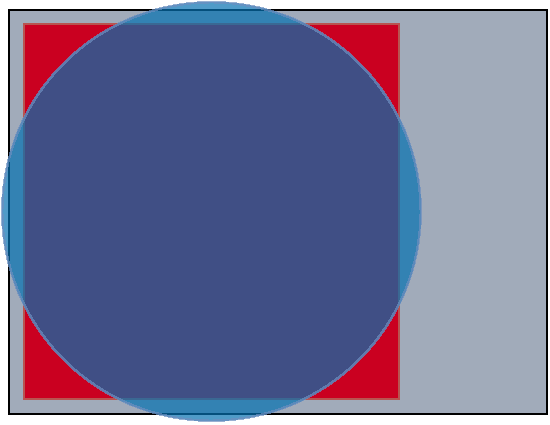
\includegraphics[width=0.7\textwidth]{media/square_vs_circle.pdf}
	 \caption{A square shape (red), as posses by a heat map, provides better space utilization on a conventional display (grey). The circle (blue) and square have the same area. A circle requires greater X and Y-axis dimensions to display the same amount of data and produces dead space at the displays corners where data cannot be presented.}
	 \label{fig:client-analysis-types}
\end{figure}

Any visualization technique used by Micromeda-Client is also challenged by the shear size of the data to be presented. For example, if all assignments for only a few organisms were displayed in the heat map described above, then its shear size would prevent users to quickly finding assignments or tracking assignments across organisms. As of version 2.0 of the Genome Properties database, there are 1296 properties and 6525 steps. If a single heat map was generated for all properties, with each cell being one 5 mm tall, such a heat map would be approximately 6.5 meters tall (i.e., fifteen vertical pages on a 24" monitor). If the same heat map was made for all property steps, the resulting heat map would be over 32.6 meters tall (i.e., seventy-five vertical pages on a 24" monitor). If both a heat map was made for both property and step assignments, the resulting heat map would be the length combined. To address this length issue, Micromeda-Client's visualization interface use interactive aggregation and de-aggregation of assignment rows to reduce the overall length of its assignment heat map.

Micromeda-Client's user interface allows users to manipulate the contents of its assignment heat map to show and hide properties and steps according to their position in the Genome Properties DAG. Because individual properties are arranged hierarchically, the assignments of properties closer to the root of the Genome Properties DAG can be used to summarize the assignments of properties closer to its leafs. In the context of a heat map, this means that a row of assignments for a parent property can be used to summarize the rows of assignments of its child properties. In addition, an assignment heat map row for a leaf genome property can be used to summarize the assignment rows of its steps. Micromeda-Client provides mechanisms expand and collapse heat map rows to display either parent summary assignments or more detailed child assignments.

\begin{figure}[!ht]
  \centering
	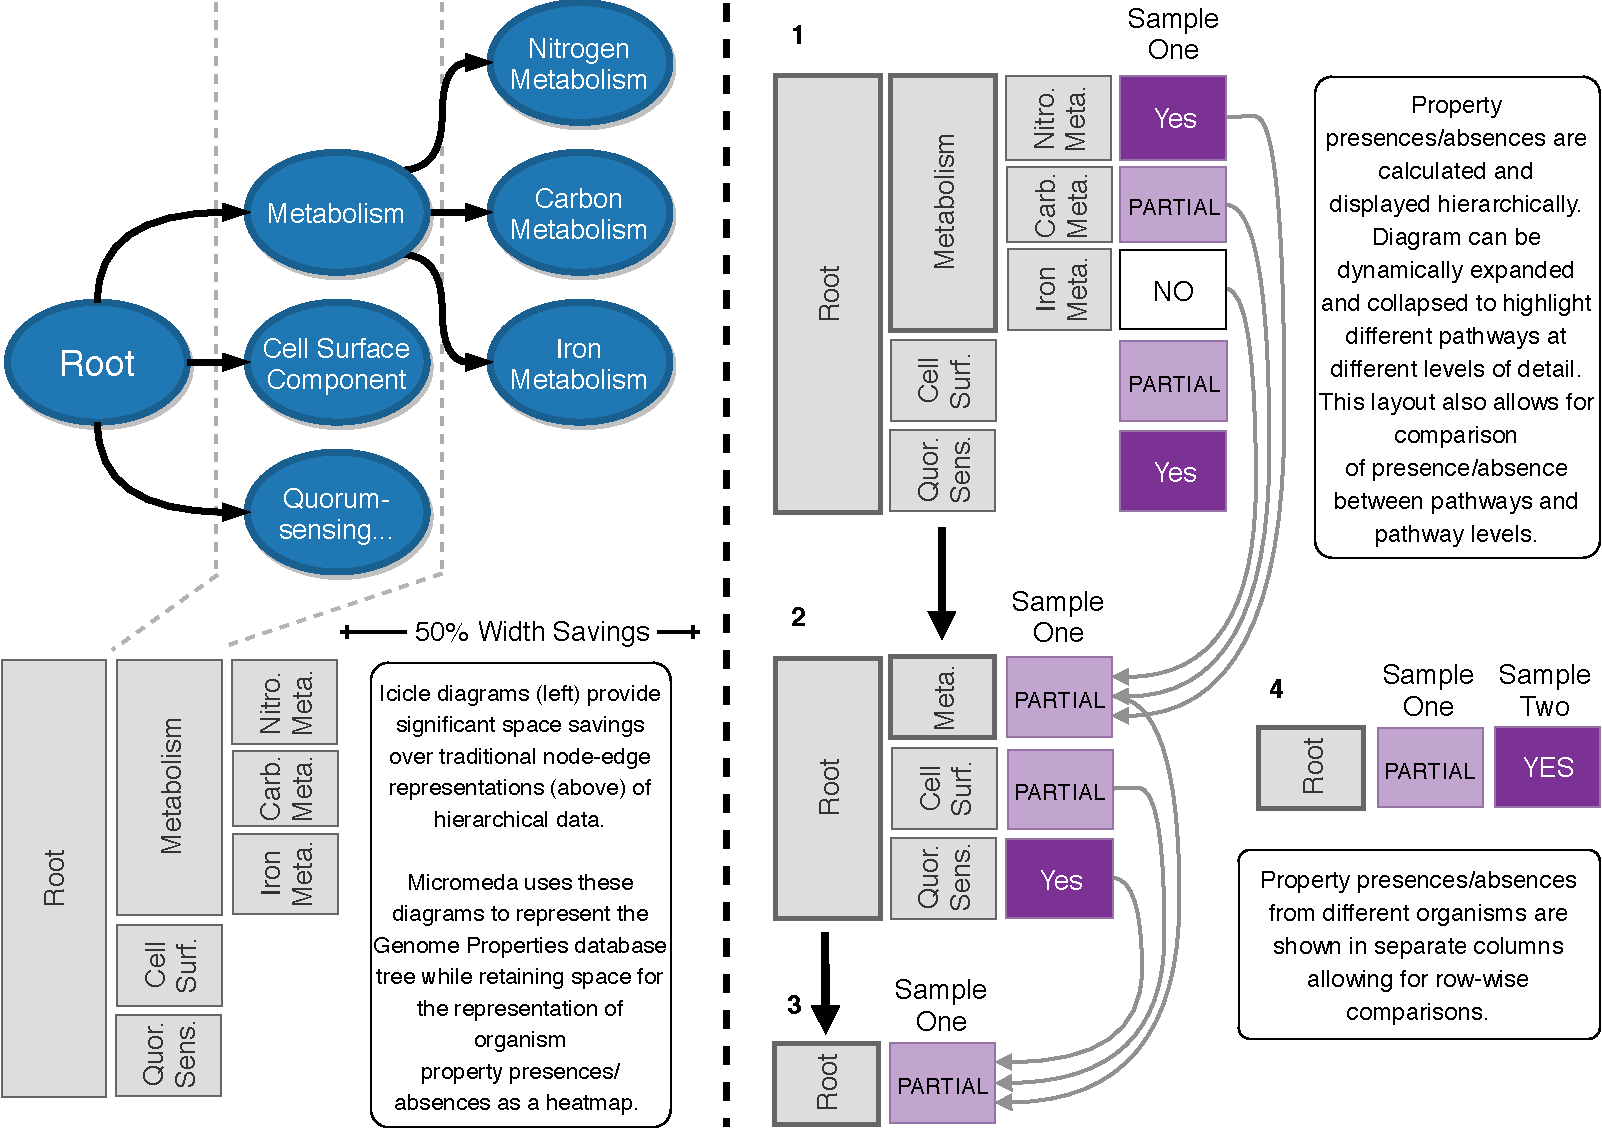
\includegraphics[width=\textwidth]{media/visualization_design_philosphy.pdf}
	 \caption{Micromeda-Client's user interface uses a clickable icicle diagram to change the state of an adjacent heat map of property and step assignments. Clicking nodes in the diagram changes the shape of the heat map by adding and removing rows from the diagram.}
	 \label{fig:visualization-philosphy}
\end{figure}

One key design decision for Micromeda-Client was how to let users control the above aggregation and de-aggregation of heat map rows. To support this usage, the author added a new visualisation component in addition to the assignment heat map. Specifically, Micromeda-Client uses a horizontal icicle diagram \footnote{Traditional icicle diagrams have leaf nodes facing downwards. The icicle diagram used by Micromeda-Client is rotated 90 degrees and has it leaf nodes facing right.} placed left of the heat map to control the heat map's row content. Icicle diagrams allow for the display of hierarchical data such as the relationship between properties or between properties and steps. Nodes which represent properties are labelled gray and those representing steps are labelled green. In Micromeda-Client, each of the genome properties and  steps in the Genome Properties database is assigned a node in the icicle diagram. The leafs of this icicle diagram are mapped to matching rows in the adjacent heat map. Icicle diagrams were chosen over other ways of visualizing hierarchical data, such as trees, due to their spacial compactness. With Micromeda-Client, the nodes in the icicle diagram are given a state of either on or off. When a node in an off state is clicked a new column added to the icicle diagram. This column's contents includes nodes representing the clicked nodes children. Simultaneously as the new child columns is added, matching assignment rows belonging to properties or steps that the child nodes represent are added and replace the clicked node's assignment row. The clicked node's shape is expanded vertically to align with the top and bottom of its first and last child node cell, respectively. If the clicked node is clicked again the process above is reversed, child nodes and their assignment rows are removed from the visualization. The clicked cell returns to its original shape and its matching summary assignment row is placed back into the heat map. Columns in the icicle diagram deleted, upon child cell removal, only if all sibling nodes to the click node do not have their children displayed.

The visualization strategy chosen for Micromeda-client supports the required tasks presented at the top of this sections. The heat map allows users to track assignments across organisms and assess their magnitude. The interactive aggregation control provided by the icicle diagram allows for the aggregation of step and property assignments into summaries. These aggregate assignments can be deaggregated to show child assignments, allowing users to explore how these aggregate assignments were derived. As the icicle diagram follows the structured of the Genome Properties DAG, specific assignments can be quickly found by following the DAG's structure from parent to child. Searching for properties is further enhanced Micromeda-Client's ability to search for properties by name. This search functionality is discussed in the next section.

\section{Additional Features of Micromeda-Client's Interface}

In addition to the visualizations capability presented above the client interface also presents several other features which help users explore their data. In the top right corner of the user interface is a text-based search box. This allows user's to search for properties by name via entering a text string. As this the user enters this string matching property names are displayed in a drop down menu. If one of these property names is clicked, then Micromeda-Client will automatically scroll to the heat map row where assignments for the property are located. If the property is not shown in the current version of the heat map, it will be added by expanding a path to the property, via recursively deaggregating parent properties along a path from the property to the root of the Genome Properties DAG.

This scrolling behaviour is also activated when a users clicks a node in the icicle diagram. When clicked the heat map will scroll to align with the top of the clicked node. As the diagram scrolls the X-axis labels remain in a fixed position to ensure columns remain labelled. 

\begin{figure}[!ht]
  \centering
	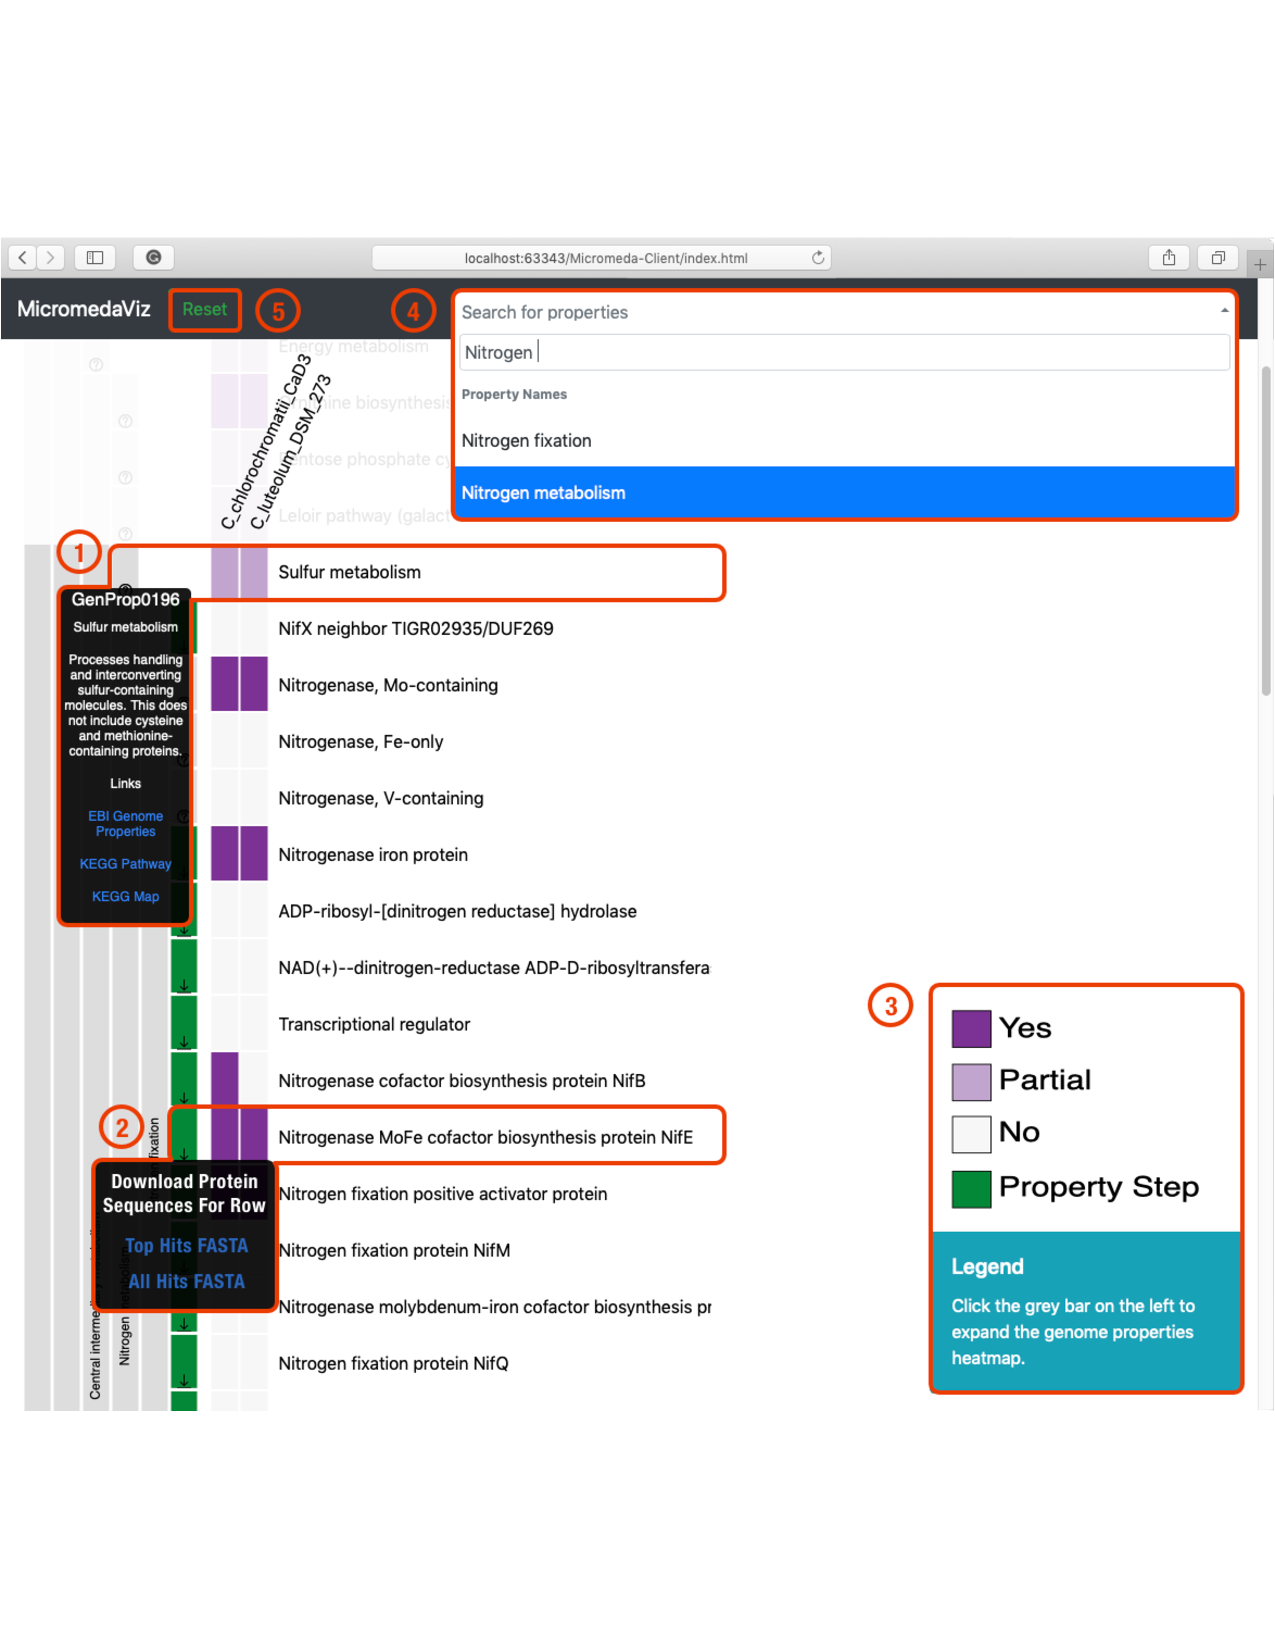
\includegraphics[width=0.9\textwidth]{media/micromeda-interface.pdf}
	 \caption{Micromeda's user interface provides functionality for searching for properties (4), getting additional information about properties and steps (1), and has the ability to download protein sequences which support step assignments (2). A legend provides context to the heat map's colours (3). A reset button allows users to reset the heat map to its initial load state(4).}
	 \label{fig:micromeda-interface}
\end{figure}

While users explore the genome property assignments of organism's in their datasets, it may be useful for them to be able to get more context about the properties whose assignments are displayed in the heat map. To facilitate this, the icicle diagram has question mark glyphs at the bottom of each node. When these glyphs are hovered over, a pop up box appears in displaying information about the property which the node represents. The pop up box includes the name of the property, a description, a link to the property in the EBI Genome Properties website, and a list of links to equivalent records in other pathways databases such as KEGG and MetaCyc. When the user's cursor leaves the glyph or the pop box, the box is once again hidden.

Property steps have different glyph at the bottom of their nodes which looks like a download symbol. It may be useful for users to download protein sequences which support the existence of property steps across organisms in an uploaded dataset. When this download download glyph is hovered over, it opens up pop up box containing two download links. The first link, when clicked, downloads a FASTA file containing the protein sequence which is most likely to carry out the step in each organism in the dataset. The second link points toward a second FASTA file containing all proteins which could carry out the step across all organisms in the dataset.

Micromeda-Client's interface also includes a reset button. This button resets the heat map and icicle diagram back to their original configuration where only top level properties are shown.

\section{Delivery Methodology}

Micromeda-Client is delivered as a client web browser application. The method was chosen due to its relative ease of deployment. End users only need open the web address of the client in order for the client to be loaded into their web browser and run. Since the application is web browser based, it will work on any operating systems with a modern web browser and even mobile devices such as tablet computers.

\section{Implementation}

Micromeda-Client's interface consists of two web pages that were structured using Hypertext Markup Language (HTML) (cite XXX), styled using Cascading Style Sheets (CSS), and scripted via Javascript (cite XXX). One page is used for uploading user generated Micromeda files and another is used for presenting the visualisation interface. To use Micromeda-Client, users must first navigate to the upload page where they can upload a Micromeda file. After upload their browser automatically redirects them to the visualisation page where they can see the contents of the uploaded file displayed in a visual manner. Both pages are styled using the Bootstrap 3.0 CSS framework (cite XXX). Boostrap is used set up page elements such as header navigation bars and drop down menus. Bootstrap also makes each of the pages compatible with tablet computers and phones as it will dynamic restyling of the above elements to a from which fits on these devices screens.

\begin{figure}[!ht]
  \centering
	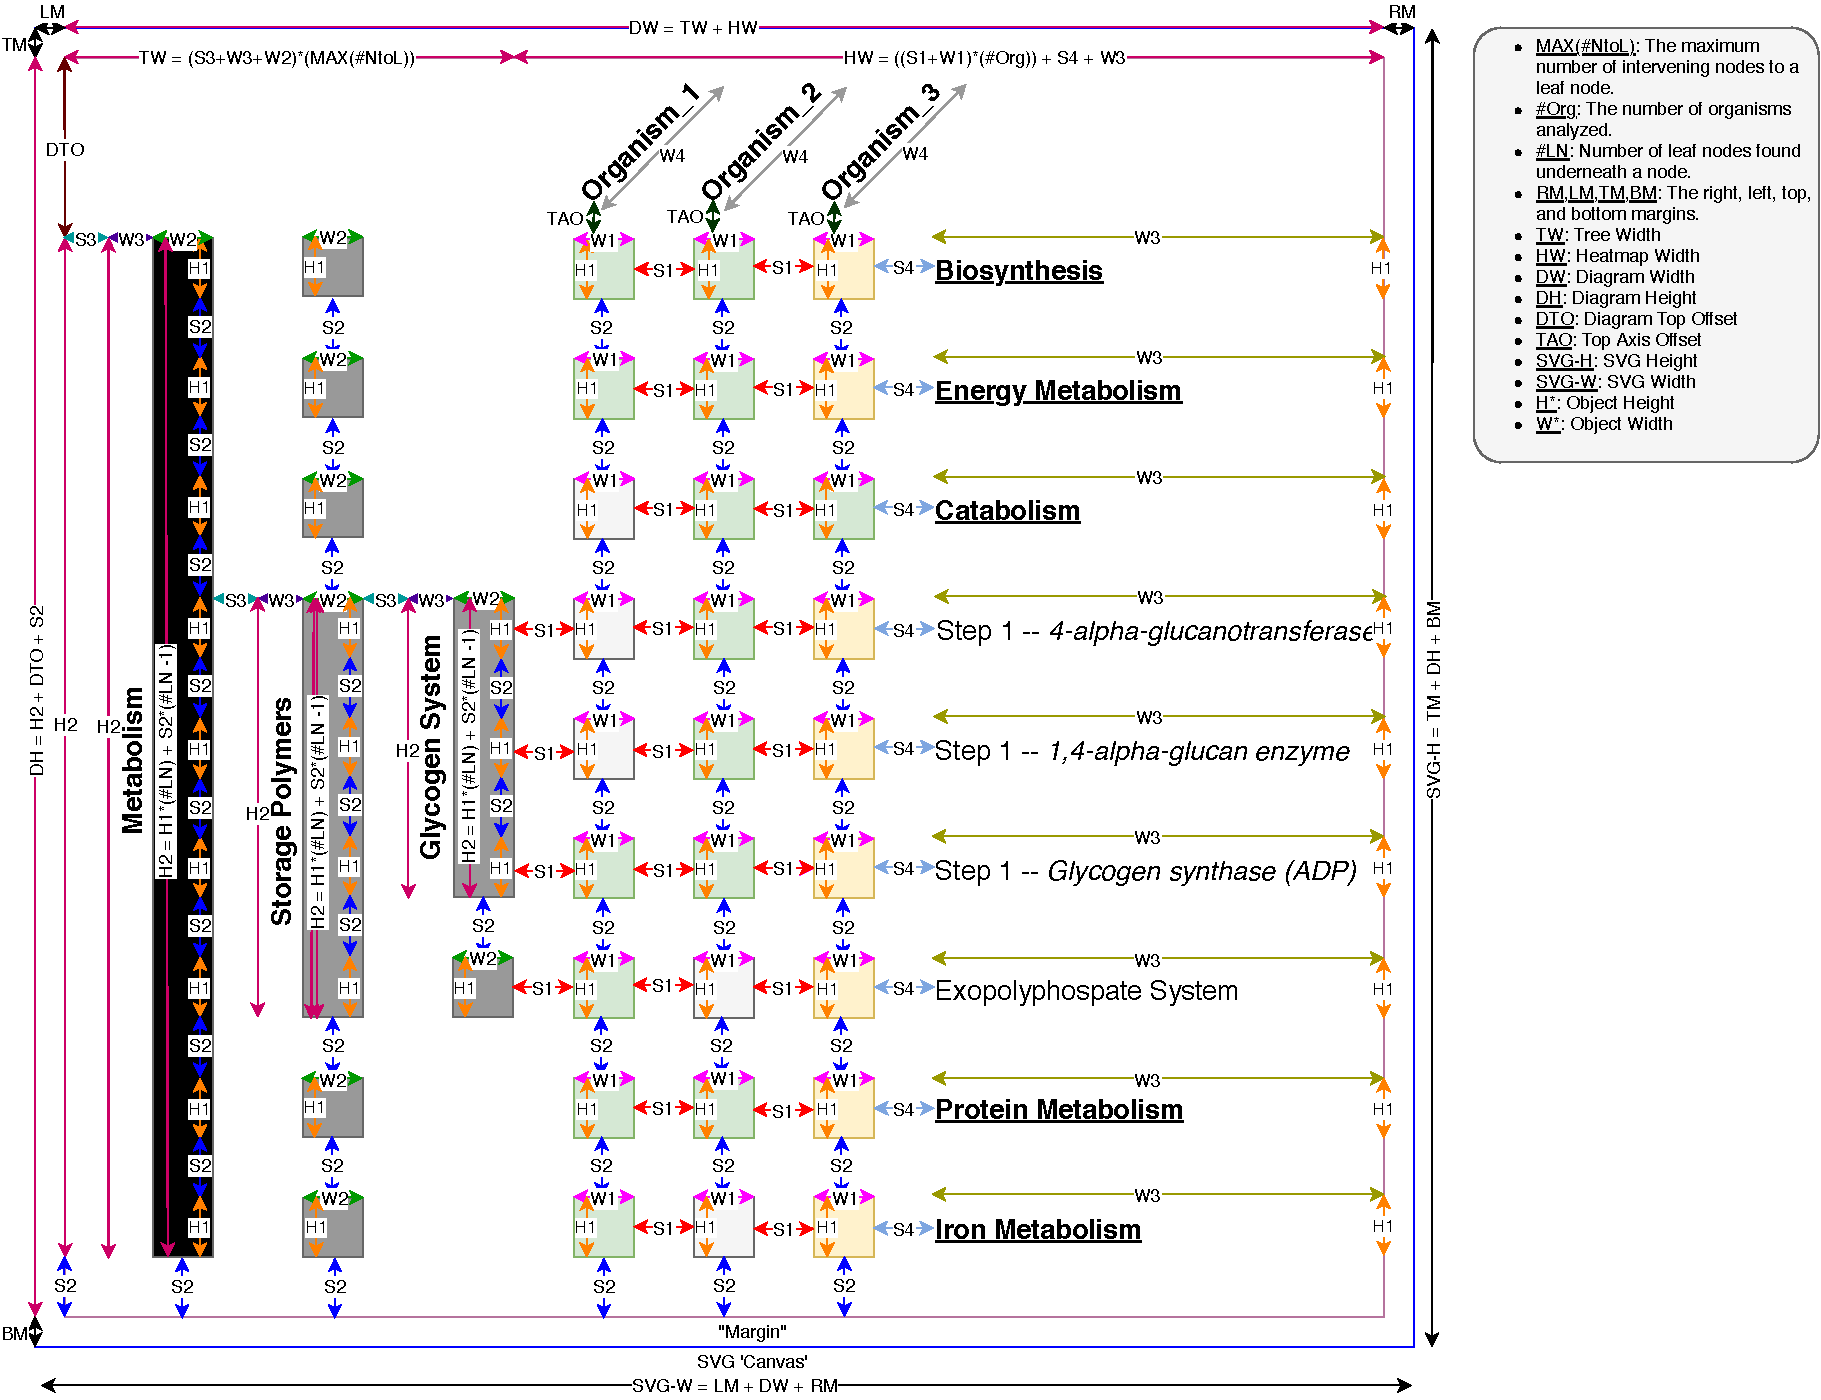
\includegraphics[width=\textwidth]{media/diagram_measurements.pdf}
	 \caption{The a series spacing, width and length values are used by Micromeda-Server to build its diagrams. These values are stored in an external file. The contents of this file can be modified to change the the layout of Micromeda-Client's visualizations.}
	 \label{fig:visualization-philosphy}
\end{figure}

Two core data structures are used by the client visualization page and they are both used during diagram generation. One is a setting array which contains a series of measurements which are used in during diagram drawing. These measurements control things like spacing between heat map cells, heat map cell dimensions and the offset of access labels. Summary of these measurements can be seen in Fig. \ref{fig:visualization-philosphy}. The second is a copy of the Genome Properties DAG in the form a tree (i.e., nodes with two parents are duplicated) of Javascript objects. Each of these objects possesses attribute, called assignments, containing a list of property assignments for a set of organisms. They also have an attribute, called enabled, containing a boolean (i.e., true or false). The contents of the visualization presented by the client directly maps to the contents of this data structure. When the property tree manipulated by the client and its diagram is then re-drawn, it is redrawn in a way that matches the new structure of the tree. The enabled boolean of each Javascript object of the aforementioned Genome Properties tree provides determines whether the children of each property should be displayed on the genome properties visualization. Properties on the tree whose enabled attribute are rendered. However, their children are not. Elements of Micromeda's user interface manipulate enabled states of objects in the property tree and this in turn can manipulate the contents of the visualization.

Diagram representing state effects.

The URL address of Micromeda-Server is found in a JSON file, called server_config.json, which is deployed along with the upload and visualization HTML files of the client. This file is loaded by both the file upload and visualization page upon load. The address below As mentioned previously, much of the functionality of Micromeda-Client is supported by Micromeda-Server. For example, the upload page contains a file drag and drop zone and when a user drops a Micromeda file on this zone it is sent from Micromeda-Client to Micromeda-Server via the server's upload endpoint. The drag and drop zone was implemented using DropzoneJS (cite XXX). After file upload is complete a dataset key is sent back the Micromeda-Server to Micromeda-Client. This dataset key is stored in the browsers site local storage (cite XXX) using a library called localForage (citeXXX) \footnote{LocalForage is a wrapper library for a variety of web browser's web local storage systems. It provides Micromeda-Client with compatibility with broader range of browsers including those with more outdated local storage systems such as the one possessed by Safari (cite XXX).} Once the dataset key is stored, the browser automatically redirects to the visualisation web page. As the visualisation page loads makes requests for a settings file, called diagram_configuration.json, from the server. This file contains 


The settings are used during visualisation generation. All requests to the server were made using the JQuery library. After this file is loaded then the client requests a JSON tree from Micromeda-Server's get\_tree endpoint using the dataset key saved in local storage. This saved key is also accessed using the indexeddb library. The server will then send back the JSON tree, which all contains assignments for all properties and steps within the Micromeda file that the dataset key points to. The visualisation is then built using the dimensions from the settings file and the data stored with in the tree JSON. The visualisations are built using D3.js library and custom Javascript library. After the visualisation generation, an interactive search menu is created in the top right hand corner of the Micromeda-Client interface. This menu is built using XXX (cite YYY).


The JSON tree loaded from the server is stored in the client as a series of interconnected Javascript objects with in the browsers. These objects form a tree structure. Each node in the tree represents a genome property or step and possesses an active attribute. This tree acts a the key data structure for Micromeda-Clients visualisation interfaces. Each node in this tree maps to a cell in the icicle diagram if the visualisation. Nodes are rendered nor not based on their parent nodes active state. When a visualisation is generated it is done so based off the data in this tree. The active attribute is used to determine if the children of this node are to be rendered during a visualisation generation. 

When a node of the icicle diagram of the visualisation is clicked it the value of this active variable's state is toggled and the entire visualisation is re-rendered. For example, when a leaf node on the icicle diagram is clicked, then the matching node in the data tree active variable is changed from false to true and then the diagram is re-rendered. During this re-rendering process the children of the clicked node are rendered. After this re-render the page is scrolled so the bottom of the x-axis labels are aligned with the top of the clicked node.

When a property name is searched for in the search menu, properties whose name is similar to the search query are displayed. When one of these menu properties are clicked then 

\section{End-User Testing}

Highlight whole rows

\section{Interface Performance}

It was found that, other then components which wait for data from Micromeda-server, all interactive components of Micormeda-Client has almost no visual lag. For example the visualisation was capable of being re-rendered almost instantaneously even when several hundred rows of assignments were needed to be displayed.

\section{Deployment}

Micromeda's user interface can can be deployed in two ways. It can be served from a web-server, such as NGINX running on the same server computer system as Micromeda-Server. Such a server is already of component of the large scale deployment of Micromeda-Server as seen in Subsection XXX. It can also be served from a content delivery network such as Amazon Cloudfront or Cloudflare. In this deployment configuration, the end user downloads the client from the geographically closest content delivery server in the the CDN, rather than the same sever as the one where Micromeda-server is hosted. After loading the client would then still send API requests to Micromeda-Server. For development purposes the files for Micromeda-Client could also be downloaded and opened by a developer's web browser.

\section{Future Improvements} \label{client-improvements}

\section{Summary} 